\chapter{Single dimension model combination\label{sec:combination}}
In chapter \ref{sec:singleDimension}, the construction of single dimension models is discussed.
These models extimate the segmentation masks of $352\times 352$ patches of scan volume slices along one of the three main axis.
In this chapter, the results of these single dimension models are combined to form a \textit{pseudo} mask that is subsequently used as labelling to train the final segmentation network.
Interesting to note in this procedure is that the evaluation metric of these obtained segmentation masks is improved in each of these steps.
The pseudo mask volume performs better than the single dimension model results and the final model trained on the pseudo masks performs better than the pseudo mask itself. 

\section{Volume combination procedure}
To construct one pseudo mask volume, first, three single dimension model are evaluated to form three stacks of two dimensional estimated segmentation masks, which are then combined to form three segmentation volumes. 
The resulting set of three segmentation volumes is then combined to form a new segmentation volume.
It is this last segmentation volume, made out of the combination, that is sliced again to obtain the pseudo masks for the final model.

\subsection{Recombination of the crops to slices}
All models are designed for $352 \times 352$ crops of the 2D slices\footnote{More information on the cropping of the slices can be found in chapter \ref{sec:cropping} on page \pageref{sec:cropping}.}.
To construct a segmentation volume from a single dimensional model, all relevant\footnote{Some slices have dimensions that do not allow to extract 5 different $352 \times 352$ crops. See for example figure \ref{fig:smallcrop} on page \pageref{fig:smallcrop}.} crops of each volume slice are evaluated.
First the segmentation results on these crops have to be combined again to obtain a segmentation mask of the whole slice.
Due to the cropping procedure, different crops of the same slice always partly overlap.
The crops are combined by averaging the logits $z_i$ for the overlapping positions.
The inferred class is then obtained from the resulting average $z_i$ values for that position. 

\subsection{Rule based result combination}
Once a stack of class segmentation masks for all slices of a volume are obtained, these can be combined to form a segmentation volumes.
Combining the results of three different single dimension models is performed in two steps:
\begin{enumerate}
    \item The resulting classification volumes are first combined with a rule-based method.
    \item After this rule-based combination, the resulting segmentation estimation is smoothened with a morphological filter.
\end{enumerate}

Three single dimension models are trained:
\begin{description}
    \item[Transverse slices] offer little context to indicate which of the lumbar vertebrae they contain. 
    It does not seem easy even for a human expert to indicate which vertebra is visible on the slice.
    The model trained on these slices is intended only for semantic segmentation.
    Each pixel is inferred only if it represents a vertebra, without distinction between the different lumbar vertebrae. 
    \item[Sagittal \& Coronal slices] do offer the necessary context to distinguish between $L_1$ to $L_5$. 
    The models trained on these slices do indicate the specific lumbar vertebra index. 
\end{description}

The volume combination rules are based on two observations:\footnote{
    The resulting estimations from a model for an input volume is again a three-dimensional volume ($\in \mathbb{N}^3$) with the same dimensions.
}.
\begin{enumerate}
    \item The precision (see equation \ref{eq:precision_i} on page \pageref{eq:precision_i}) with which the background class is predicted in all models is very high.
            This means $\mathcal{P} \left( label = background \mid prediction = background \right)$ is high for all models. 
            If there is one model that indicates a position is background, this position could be estimated to be background with high probability.
    \item The rule mentioned above can be nuanced\footnote{The opportunity to use the results of the other two single dimension models to correct a \textit{lapse} of one of the single dimension models can be recognized as one of the strengths of the combination procedure.}.
    It was observed that single dimension models can miss the mask\footnote{This is caused by the large differences between the different datasets used, see chapter \ref{sec:datasets} at page \pageref{sec:datasets}.}. 
    For some volumes, the recall of the vertebra class is extremely low. The single dimension model predicts the background class for allmost all positions.
    When this is observed, it does not make much sense to stick to the first rule.
\end{enumerate}
The observations mentioned above can be combined in algorithm \ref{alg:combination}.

\subsection{Morphological smoothing}
After the rule-based combination of estimations from different single dimension models, the result is smoothened with standard morphological filters.
These filters are combinations of the morphological \textit{erosion} and \textit{dilation} operators\footnote{
    This document is not intended to provide an elaborate explanation on morphological operations.
    For the readers conventience, the following symbolic notations are repeated:
    \begin{description}
        \item[Erosion] of set $\mathbf{A}$ by structural element $\mathbf{B}$ : $\mathbf{A} \ominus \mathbf{B}$ 
        \item[Dilation] of set $\mathbf{A}$ by structural element $\mathbf{B}$ : $\mathbf{A} \oplus \mathbf{B}$ 
        \item[Opening] of set $\mathbf{A}$ by structural element $\mathbf{B}$ : $\mathbf{A} \circ \mathbf{B} = (\mathbf{A} \ominus \mathbf{B}) \oplus \mathbf{B}$
        \item[Closing] of set $\mathbf{A}$ by structural element $\mathbf{B}$ : $\mathbf{A} \bullet \mathbf{B} = (\mathbf{A} \oplus \mathbf{B}) \ominus \mathbf{B}$
    \end{description}
}.

\begin{itemize}
    \item Noise in the single dimension segmentation masks is suppressed with an opening operation on the individual segmentation volumes of the single dimension models.
    \item Noise in the combined volumes is suppressed by first opening and then closing the volumes.
    \item The estimated volumes are observed to overestimate the extent of the vertebrae. For this reason, an erosion step is performed to decrease the overall extent of the class masks.
\end{itemize}

The procedure mentioned above has two hyperparameters: the number of iterations for the denoising filters and the number of iterations for the erosion filter.
Both hyperparameters are estimated by calculating the same evaluation metric, the weighted dice score on the validation set, as for the single-dimensional model evaluation. 

\subsection{Volume combination algorithm}
The combination of the rules and morphological smoothing operations discussed above result in the following algorithm to combine the segmentation volumes from the single dimension models\footnote{
    The cardinality of a set $\mathbf{A}$, written as $|\mathbf{A}|$, is the number of elements in a set.
    The cardinality of the class label sets $c_.$ thus represents the voxel count in each segmentation volumes that is estimated to be \textit{not background}.
    Suspiciously low voxel counts classified other than background are defined as lower than 35\% of the highest class label cardinality.
    This last factor has not been optimised. It is an engineering estimate.
    If a volume is found to be have such a low class label cardinality, this volume reference is stored as $d_{ignore}$ and the volume is ignore in the combination protocol.
    In practice, the low cardinality volumes are all the segmentation volumes obtained from the model trained on point annotated tranverse slices.
}:

\begin{algorithm}[H]
    \SetAlgoLined
    \KwData{
        Results $y_.$ of three models indicating an estimated class for all positions $\vec{p}$ in the volume. \;
        Transverse model $y_t \in \mathbb{N}^3: \forall y_t(\vec{p}) \in \{ 0, 1 \}$ \;
        Sagittal model $y_s \in \mathbb{N}^3: \forall y_t(\vec{p}) \in \{ 0, 1, 2, 3, 4, 5 \}$ \;
        Coronal model $y_c \in \mathbb{N}^3: \forall y_t(\vec{p}) \in \{ 0, 1, 2, 3, 4, 5 \}$  \;
        Binary $\mathbf{B}$ structure with rank 3 and connectivity 3 \;
    }
    \KwResult{Combination of the three model results $y_f$.}
    \tcp{Closing operation on all $y_.$}
    $y_t \leftarrow y_t \bullet \mathbf{B}$ \;
    $y_s \leftarrow y_s \bullet \mathbf{B}$ \;
    $y_c \leftarrow y_c \bullet \mathbf{B}$ \;
    \tcp{(relative) cardinality of the class label sets}
    $c_t \leftarrow |\{ y_t \neq 0 \}|$ \;
    $c_s \leftarrow |\{ y_s \neq 0 \}|$ \;
    $c_c \leftarrow |\{ y_c \neq 0 \}|$ \;
    $r_t \leftarrow \frac{c_t}{max(c_t, c_s, c_c)}$ \;
    $r_s \leftarrow \frac{c_s}{max(c_t, c_s, c_c)}$ \;
    $r_c \leftarrow \frac{c_c}{max(c_t, c_s, c_c)}$ \;
    \lIf{$\exists d \in [ t,s,c ] : r_d < 0.35$}{$d_{ignore} \leftarrow d$}\lElse{$d_{ignore} \leftarrow \emptyset$}
    \For{all $\vec{p}$}{
        $i \in [ 1, 2, 3, 4, 5]$ \;
        \Switch{$d_{ignore}$}{
            \Case{$\emptyset$}{
                \lIf{$y_t[\vec{p}] = 1 \wedge y_s[\vec{p}] = i \wedge y_c[\vec{p}] = i$}{
                    $y_f[\vec{p}] \leftarrow i$ 
                }
                \lElse{
                    $y_f[\vec{p}] \leftarrow 0$ 
                }
            }
            \Case{$t$}{
                \lIf{$y_s[\vec{p}] = i \wedge y_c[\vec{p}] = i$}{
                    $y_f[\vec{p}] \leftarrow i$ 
                }
                \lElse{
                    $y_f[\vec{p}] \leftarrow 0$
                }
            }
            \Case{$s$}{
                \lIf{$y_t[\vec{p}] = 1 \wedge y_c[\vec{p}] = i$}{
                    $y_f[\vec{p}] \leftarrow i$ 
                }
                \lElse{
                    $y_f[\vec{p}] \leftarrow 0$ 
                }
            }
            \Case{$c$}{
                \lIf{$y_t[\vec{p}] = 1 \wedge y_s[\vec{p}] = i$}{
                    $y_f[\vec{p}] \leftarrow i$ 
                }
                \lElse{
                    $y_f[\vec{p}] \leftarrow 0$ 
                }
            }
        }
    }
    $y_f \leftarrow ((y_f \circ \mathbf{B}) \bullet \mathbf{B}) \ominus \mathbf{B}$
   \caption{Rule based combination of model results from three single dimension models\label{alg:combination}}
\end{algorithm}Only one semantic class is estimated in the first row, illustrating the model trained on transversal slices.
On the first three rows, slices of the resulting segmentations from the single dimension models are shown. 
It is clear these masks contain some artefacts and are not always in agreement with each other.
On the fourth row, the result after mask combination and morphological smoothing is shown. 
This corresponds more closely to the ground truth mask, shown on the fifth row.
This final mask, shown on the fourth row, will be used as a pseudo mask to approximate the unknown ground truth mask.
In the last row, the corresponding images are shown.

\begin{SCtable}[\sidecaptionrelwidth][h]

    \begin{tabular}{l|lll}
        \hline
        \textbf{\begin{tabular}[c]{@{}l@{}}Slice \\ direction\end{tabular}} &
          \textbf{Transverse} &
          \textbf{Coronal} &
          \textbf{Sagittal} \\ \hline
        \begin{tabular}[c]{@{}l@{}}Context\\ Slices {[}mm{]}\end{tabular}           & 1      & 1      & 1      \\ \cline{1-1}
        \begin{tabular}[c]{@{}l@{}}Points per\\ class instance\end{tabular}         & 1      & 1      & 1      \\ \cline{1-1}
        \begin{tabular}[c]{@{}l@{}}Background \\ points\end{tabular}                & 5      & 3      & 3      \\ \cline{1-1}
        Dataset &
          \begin{tabular}[c]{@{}l@{}}PLoS\\ xVertSeg\\ USiegen\\ MyoSegmenTUM\end{tabular} &
          \multicolumn{2}{l}{\begin{tabular}[c]{@{}l@{}}xVertSeg\\ USiegen\\ MyoSegmenTUM\end{tabular}} \\ \cline{1-1}
        \begin{tabular}[c]{@{}l@{}}Segmentation\\ classes\end{tabular}              & 2      & 6      & 6      \\ \cline{1-1}
        \begin{tabular}[c]{@{}l@{}}Weighted \\ dice score\end{tabular}              & 0.46   & 0.38   & 0.38   \\ \hline
        \begin{tabular}[c]{@{}l@{}}Weighted\\ dice score\\ combination\end{tabular} & \multicolumn{3}{c}{0.51} \\ \hline
        \end{tabular}
    \caption{Combination of three point supervised models with algorithm \ref{alg:combination}. 
    These models were constructed with a fixed number of background points and a fixed number of class labels per class instance.
    This test indicates that the segmentation mask obtained from the result of single dimension models with algorithm \ref{alg:combination} allows to obtain a new segmentation mask with a higher metric score, the pseudo masks.
    The weighted dice scores are evaluated on the cross validation set, this causes the difference with the values in figure \ref{fig:points_influence}. \label{tab:combination_1}
    }

\end{SCtable}
\par{
    In table \ref{tab:combination_1}, the segmentation quality is calculated on the validation set.
    Since there are two hyperparameters (the number of denoise iterations and the number of erosion iterations) to optimise in the combination algorithm \ref{alg:combination}, 
    the algorithm is evaluated with a matrix of these hyperparameters to choose the optimal hyperparameter set to construct the pseudo masks for the test set.
    In figure \ref{fig:hyperparameter_combination_1}, this obtimization procedure is illustrated.
    The optimal hyperparameter set in this case was 2 denoise iterations and 1 erosion iteration.
}
\marginpar{
        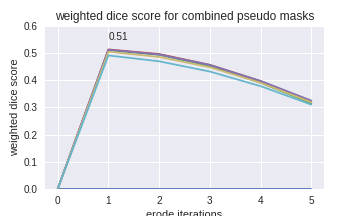
\includegraphics[width=5cm]{images/combination_optimization_1.png}
        \captionof{figure}{Illustration of the hyperparameter optimization procedure for the combination detailed in \ref{tab:combination_1}}
        \label{fig:hyperparameter_combination_1}
    }
\par{
    The result of this procedure is illustrated in figures \ref{fig:comb1_1} and \ref{fig:comb1_2}.
    In the second figure, the model trained on transversal slices is predicting almost exclusively background labels.
    The check in algorithm \ref{alg:combination} for volume class cardinality is usefule in this type of cases.
}   
\par{
    The procedure described in the last two chapters now allows to train a network with only point annotated labels by using the results of the pseudo mask volume.
    Mind however that the results in chapter \ref{sec:singleDimension} and the results combined in this chapter were obtained with a different set of point annotations for each dimension.
    This was done to make comparison possible.
}
\par{
    In reality, an expert will generate a single stack of annotations, not three.
    As described in chapter \ref{sec:annotationPoints} on page \pageref{sec:annotationPoints}, one of the single dimensional models will be trained on this stack of annotated slices.
    The other two however, will be trained on stacks where the same annotation points are used, but now as these are found back when slicing in the two other dimensions.
}

\begin{SCfigure}[][htb]
    \centering
    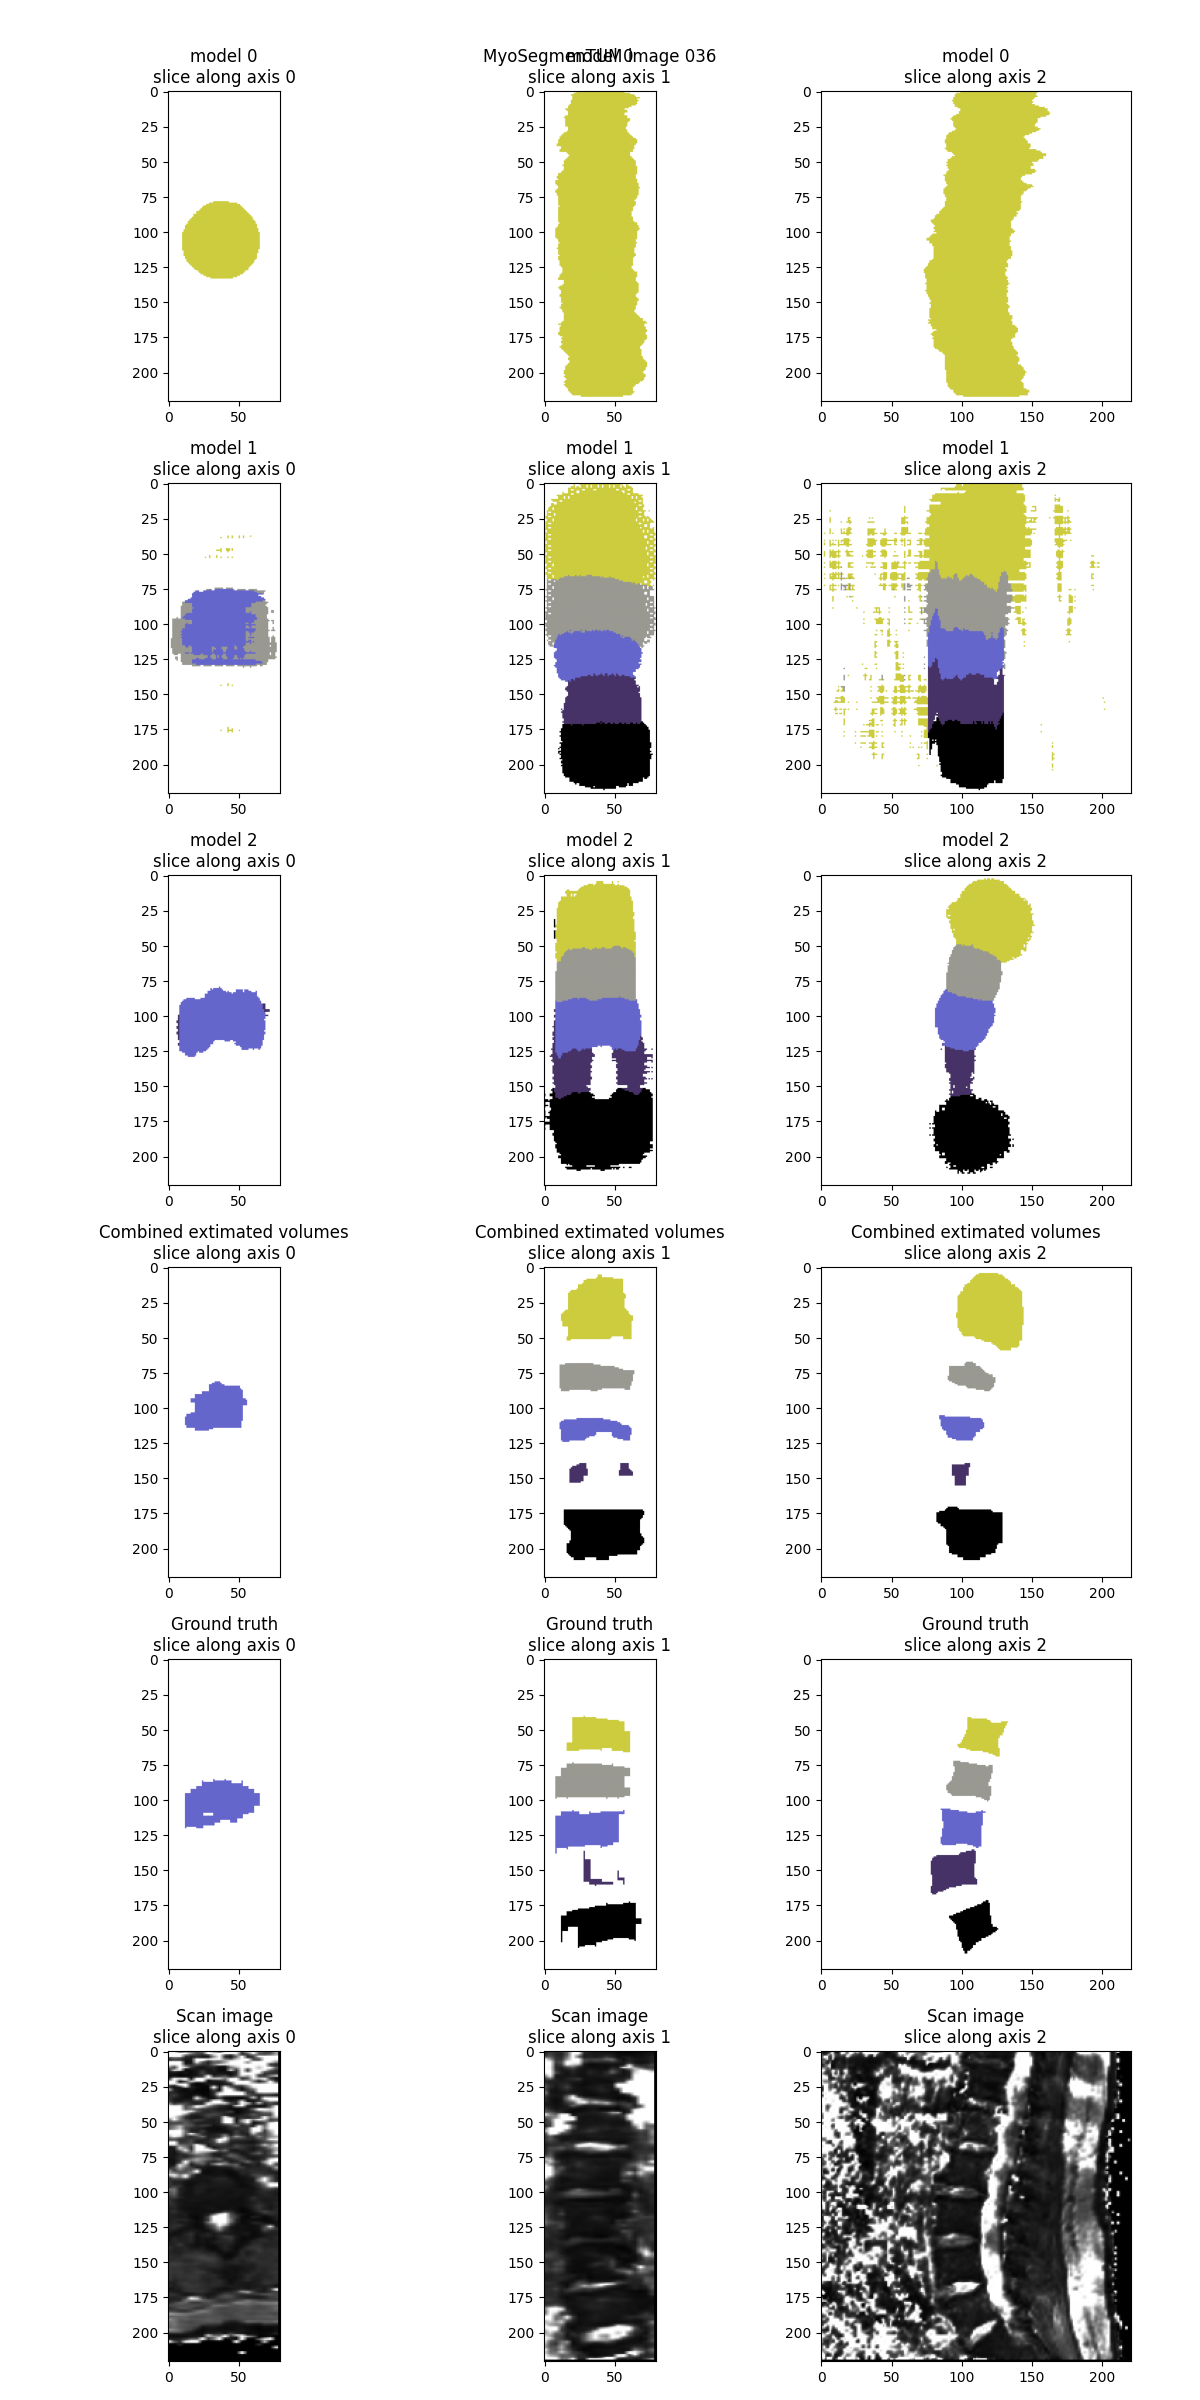
\includegraphics[width=.95\textwidth]{images/comb1_denoise2_erode1_MyoSegmenTUM_036.png}
    \caption{
        Result of the combination of the three single dimension model results for volume MyoSegmenTUM nr 36.
        The colours indicate the vertebra classes. Only one semantic class is estimated in the first row, illustrating the model trained on transversal slices.
        On the first three rows, slices of the resulting segmentations from the single dimension models are shown. 
        It is clear these masks contain some artefacts and are not always in agreement with each other.
        On the fourth row, the result after mask combination and morphological smoothing is shown. 
        This corresponds more closely to the ground truth mask, shown on the fifth row.
        This final mask, shown on the fourth row, will be used as a pseudo mask to approximate the unknown ground truth mask.
        In the last row, the corresponding images are shown. \label{fig:comb1_1}
    }
\end{SCfigure}
\begin{SCfigure}[][htb]
    \centering
    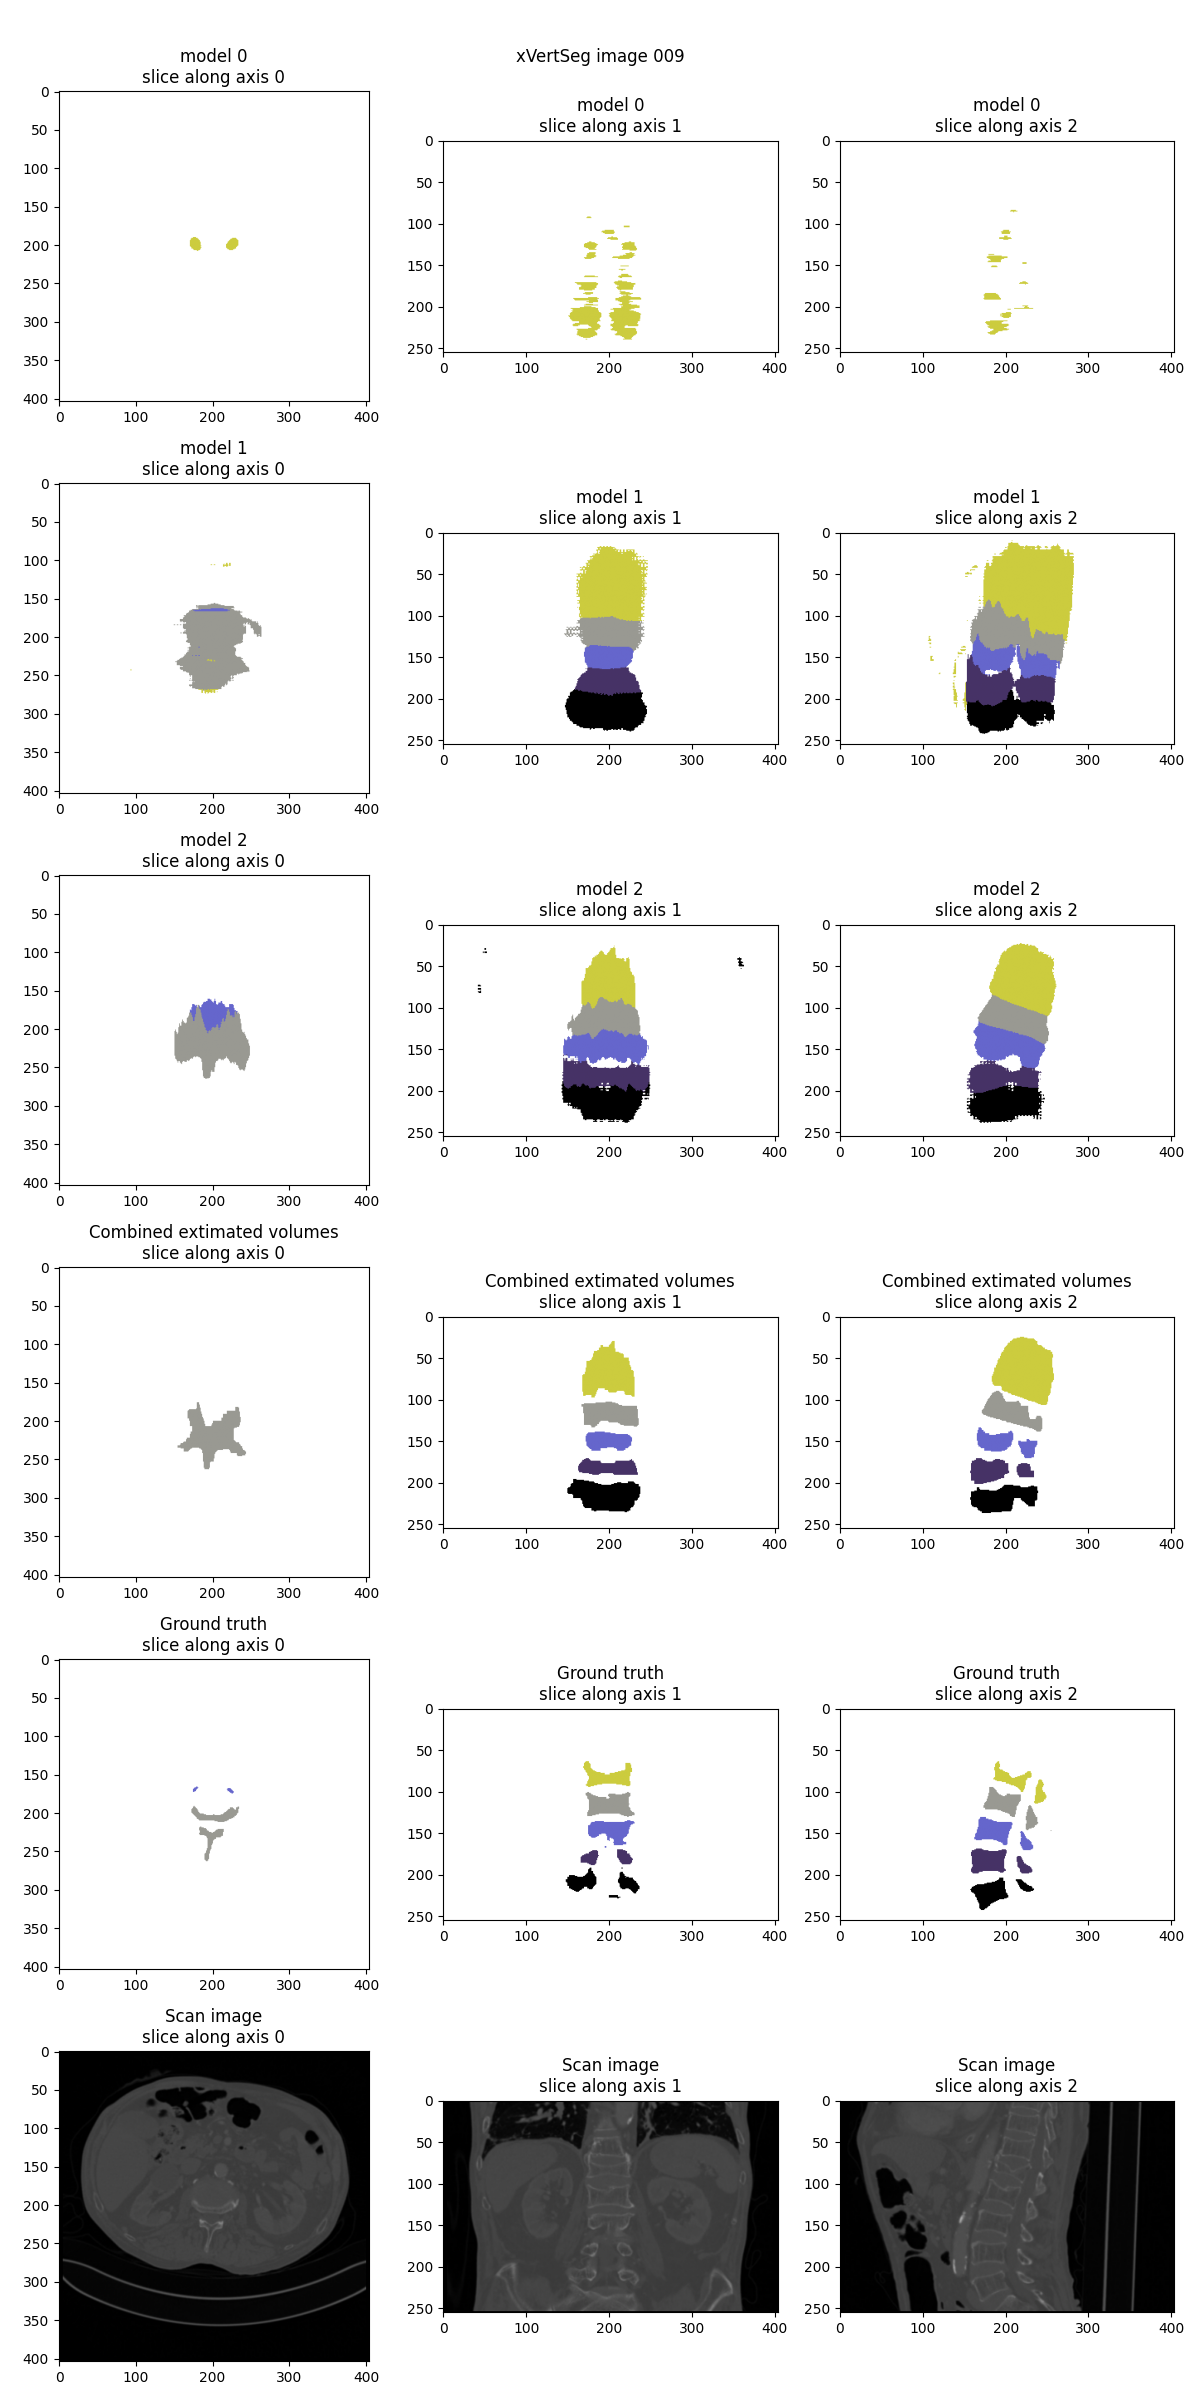
\includegraphics[width=.95\textwidth]{images/comb1_denoise2_erode1_xVertSeg_009.png}
    \caption{
        Result of the combination of the three single dimension model results for volume xVertSeg 009.
        The colours indicate the vertebra classes. The layout of this image is the same as the layout of figure \ref{fig:comb1_1}.
        This image illustrates a case where the usefulness of the rule in algorithm \ref{alg:combination}  to ignore a single dimension model result with a cardinality 
        of the class set under 35\% of the max value is shown.\label{fig:comb1_2}
    }
\end{SCfigure}

\chapter{Pseudo mask training}

\par{
    As described in chapter \ref{sec:annotationPoints} on page \pageref{sec:annotationPoints}, only one stack of slices will be annotated by the expert.
    This means that for the slices along one of the geometric dimensions, a 
}



\begin{SCtable}[\sidecaptionrelwidth][h]

    \begin{tabular}{l|lll}
        \hline
        \textbf{\begin{tabular}[c]{@{}l@{}}Slice \\ direction\end{tabular}} &
          \textbf{Transverse} &
          \textbf{Coronal} &
          \textbf{Sagittal} \\ \hline
        \begin{tabular}[c]{@{}l@{}}Context\\ Slices {[}mm{]}\end{tabular}           & 1        & 1        & 1    \\ \cline{1-1}
        \begin{tabular}[c]{@{}l@{}}Points per\\ class instance\end{tabular}         & variable & variable & 3    \\ \cline{1-1}
        \begin{tabular}[c]{@{}l@{}}Background \\ points\end{tabular}                & variable & variable & 5    \\ \cline{1-1}
        Dataset &
          \begin{tabular}[c]{@{}l@{}}PLoS\\ xVertSeg\\ USiegen\\ MyoSegmenTUM\end{tabular} &
          \multicolumn{2}{l}{\begin{tabular}[c]{@{}l@{}}xVertSeg\\ USiegen\\ MyoSegmenTUM\end{tabular}} \\ \cline{1-1}
        \begin{tabular}[c]{@{}l@{}}Segmentation\\ classes\end{tabular}              & 2        & 6        & 6    \\ \cline{1-1}
        \begin{tabular}[c]{@{}l@{}}Weighted \\ dice score\end{tabular}              & 0.00     & 0.00     & 0.00 \\ \hline
        \begin{tabular}[c]{@{}l@{}}Weighted\\ dice score\\ combination\end{tabular} & \multicolumn{3}{c}{0.00}   \\ \hline
        \end{tabular}
    \caption{Combination of three point supervised models with algorithm \ref{alg:combination}. 
    These models were constructed with a fixed number of background points and a fixed number of class labels per class instance.
    This test indicates that the segmentation mask obtained from the result of single dimension models with algorithm \ref{alg:combination} allows to obtain a new segmentation mask with a higher metric score, the pseudo masks.
    The weighted dice scores are evaluated on the cross validation set, this causes the difference with the values in figure \ref{fig:points_influence}. \label{tab:combination_1}
    }

\end{SCtable}

Time to evaluate
performance